\documentclass[twoside]{book}

% Packages required by doxygen
\usepackage{fixltx2e}
\usepackage{calc}
\usepackage{doxygen}
\usepackage[export]{adjustbox} % also loads graphicx
\usepackage{graphicx}
\usepackage[utf8]{inputenc}
\usepackage{makeidx}
\usepackage{multicol}
\usepackage{multirow}
\PassOptionsToPackage{warn}{textcomp}
\usepackage{textcomp}
\usepackage[nointegrals]{wasysym}
\usepackage[table]{xcolor}

% Font selection
\usepackage[T1]{fontenc}
\usepackage[scaled=.90]{helvet}
\usepackage{courier}
\usepackage{amssymb}
\usepackage{sectsty}
\renewcommand{\familydefault}{\sfdefault}
\allsectionsfont{%
  \fontseries{bc}\selectfont%
  \color{darkgray}%
}
\renewcommand{\DoxyLabelFont}{%
  \fontseries{bc}\selectfont%
  \color{darkgray}%
}
\newcommand{\+}{\discretionary{\mbox{\scriptsize$\hookleftarrow$}}{}{}}

% Page & text layout
\usepackage{geometry}
\geometry{%
  a4paper,%
  top=2.5cm,%
  bottom=2.5cm,%
  left=2.5cm,%
  right=2.5cm%
}
\tolerance=750
\hfuzz=15pt
\hbadness=750
\setlength{\emergencystretch}{15pt}
\setlength{\parindent}{0cm}
\setlength{\parskip}{3ex plus 2ex minus 2ex}
\makeatletter
\renewcommand{\paragraph}{%
  \@startsection{paragraph}{4}{0ex}{-1.0ex}{1.0ex}{%
    \normalfont\normalsize\bfseries\SS@parafont%
  }%
}
\renewcommand{\subparagraph}{%
  \@startsection{subparagraph}{5}{0ex}{-1.0ex}{1.0ex}{%
    \normalfont\normalsize\bfseries\SS@subparafont%
  }%
}
\makeatother

% Headers & footers
\usepackage{fancyhdr}
\pagestyle{fancyplain}
\fancyhead[LE]{\fancyplain{}{\bfseries\thepage}}
\fancyhead[CE]{\fancyplain{}{}}
\fancyhead[RE]{\fancyplain{}{\bfseries\leftmark}}
\fancyhead[LO]{\fancyplain{}{\bfseries\rightmark}}
\fancyhead[CO]{\fancyplain{}{}}
\fancyhead[RO]{\fancyplain{}{\bfseries\thepage}}
\fancyfoot[LE]{\fancyplain{}{}}
\fancyfoot[CE]{\fancyplain{}{}}
\fancyfoot[RE]{\fancyplain{}{\bfseries\scriptsize Generated by Doxygen }}
\fancyfoot[LO]{\fancyplain{}{\bfseries\scriptsize Generated by Doxygen }}
\fancyfoot[CO]{\fancyplain{}{}}
\fancyfoot[RO]{\fancyplain{}{}}
\renewcommand{\footrulewidth}{0.4pt}
\renewcommand{\chaptermark}[1]{%
  \markboth{#1}{}%
}
\renewcommand{\sectionmark}[1]{%
  \markright{\thesection\ #1}%
}

% Indices & bibliography
\usepackage{natbib}
\usepackage[titles]{tocloft}
\setcounter{tocdepth}{3}
\setcounter{secnumdepth}{5}
\makeindex

% Hyperlinks (required, but should be loaded last)
\usepackage{ifpdf}
\ifpdf
  \usepackage[pdftex,pagebackref=true]{hyperref}
\else
  \usepackage[ps2pdf,pagebackref=true]{hyperref}
\fi
\hypersetup{%
  colorlinks=true,%
  linkcolor=blue,%
  citecolor=blue,%
  unicode%
}

% Custom commands
\newcommand{\clearemptydoublepage}{%
  \newpage{\pagestyle{empty}\cleardoublepage}%
}

\usepackage{caption}
\captionsetup{labelsep=space,justification=centering,font={bf},singlelinecheck=off,skip=4pt,position=top}

%===== C O N T E N T S =====

\begin{document}

% Titlepage & ToC
\hypersetup{pageanchor=false,
             bookmarksnumbered=true,
             pdfencoding=unicode
            }
\pagenumbering{alph}
\begin{titlepage}
\vspace*{7cm}
\begin{center}%
{\Large My Project }\\
\vspace*{1cm}
{\large Generated by Doxygen 1.8.13}\\
\end{center}
\end{titlepage}
\clearemptydoublepage
\pagenumbering{roman}
\tableofcontents
\clearemptydoublepage
\pagenumbering{arabic}
\hypersetup{pageanchor=true}

%--- Begin generated contents ---
\chapter{File Index}
\section{File List}
Here is a list of all files with brief descriptions\+:\begin{DoxyCompactList}
\item\contentsline{section}{\hyperlink{bleprph_8h}{bleprph.\+h} }{\pageref{bleprph_8h}}{}
\item\contentsline{section}{\hyperlink{gatt__svr_8c}{gatt\+\_\+svr.\+c} }{\pageref{gatt__svr_8c}}{}
\item\contentsline{section}{\hyperlink{main_8c}{main.\+c} }{\pageref{main_8c}}{}
\item\contentsline{section}{\hyperlink{misc_8c}{misc.\+c} }{\pageref{misc_8c}}{}
\end{DoxyCompactList}

\chapter{File Documentation}
\hypertarget{bleprph_8h}{}\section{bleprph.\+h File Reference}
\label{bleprph_8h}\index{bleprph.\+h@{bleprph.\+h}}
{\ttfamily \#include \char`\"{}log/log.\+h\char`\"{}}\newline
{\ttfamily \#include \char`\"{}nimble/ble.\+h\char`\"{}}\newline
Include dependency graph for bleprph.\+h\+:
\nopagebreak
\begin{figure}[H]
\begin{center}
\leavevmode
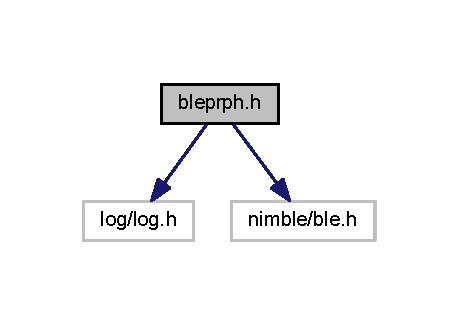
\includegraphics[width=220pt]{bleprph_8h__incl}
\end{center}
\end{figure}
This graph shows which files directly or indirectly include this file\+:
\nopagebreak
\begin{figure}[H]
\begin{center}
\leavevmode
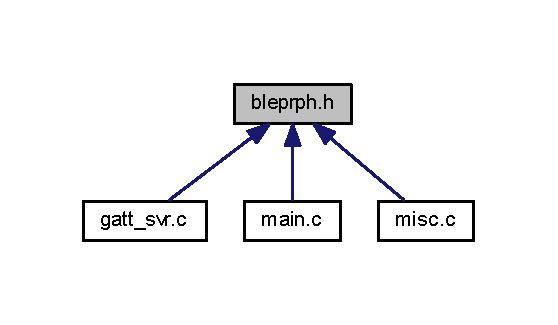
\includegraphics[width=268pt]{bleprph_8h__dep__incl}
\end{center}
\end{figure}
\subsection*{Macros}
\begin{DoxyCompactItemize}
\item 
\#define \hyperlink{bleprph_8h_aefef1b46188d31d675109172c8fea541}{B\+L\+E\+P\+R\+P\+H\+\_\+\+L\+O\+G\+\_\+\+M\+O\+D\+U\+LE}~(L\+O\+G\+\_\+\+M\+O\+D\+U\+L\+E\+\_\+\+P\+E\+R\+U\+S\+ER + 0)
\item 
\#define \hyperlink{bleprph_8h_a0107941128bc824a416d3708c2dee708}{B\+L\+E\+P\+R\+P\+H\+\_\+\+L\+OG}(lvl, ...)~L\+O\+G\+\_\+ \#\# lvl(\&\hyperlink{main_8c_a3cb7621a683b5c12e82853697f64aafb}{bleprph\+\_\+log}, \hyperlink{bleprph_8h_aefef1b46188d31d675109172c8fea541}{B\+L\+E\+P\+R\+P\+H\+\_\+\+L\+O\+G\+\_\+\+M\+O\+D\+U\+LE}, \+\_\+\+\_\+\+V\+A\+\_\+\+A\+R\+G\+S\+\_\+\+\_\+)
\item 
\#define \hyperlink{bleprph_8h_a584c8254368412ed90d78cf12bd99be7}{G\+A\+T\+T\+\_\+\+S\+V\+R\+\_\+\+S\+V\+C\+\_\+\+A\+L\+E\+R\+T\+\_\+\+U\+U\+ID}~0x1811
\item 
\#define \hyperlink{bleprph_8h_ad3a7580a1792cabd6ddbe36f2531d1a9}{G\+A\+T\+T\+\_\+\+S\+V\+R\+\_\+\+C\+H\+R\+\_\+\+S\+U\+P\+\_\+\+N\+E\+W\+\_\+\+A\+L\+E\+R\+T\+\_\+\+C\+A\+T\+\_\+\+U\+U\+ID}~0x2\+A47
\item 
\#define \hyperlink{bleprph_8h_aa44e336db19e3d1e975792f725f432b5}{G\+A\+T\+T\+\_\+\+S\+V\+R\+\_\+\+C\+H\+R\+\_\+\+N\+E\+W\+\_\+\+A\+L\+E\+RT}~0x2\+A46
\item 
\#define \hyperlink{bleprph_8h_a425fcbd9c1f701b7f04bc6d0df767412}{G\+A\+T\+T\+\_\+\+S\+V\+R\+\_\+\+C\+H\+R\+\_\+\+S\+U\+P\+\_\+\+U\+N\+R\+\_\+\+A\+L\+E\+R\+T\+\_\+\+C\+A\+T\+\_\+\+U\+U\+ID}~0x2\+A48
\item 
\#define \hyperlink{bleprph_8h_acd1dec23d1dc0c703bd83431180d3c25}{G\+A\+T\+T\+\_\+\+S\+V\+R\+\_\+\+C\+H\+R\+\_\+\+U\+N\+R\+\_\+\+A\+L\+E\+R\+T\+\_\+\+S\+T\+A\+T\+\_\+\+U\+U\+ID}~0x2\+A45
\item 
\#define \hyperlink{bleprph_8h_a1a85783a764577d4e89f0896fe1cb884}{G\+A\+T\+T\+\_\+\+S\+V\+R\+\_\+\+C\+H\+R\+\_\+\+A\+L\+E\+R\+T\+\_\+\+N\+O\+T\+\_\+\+C\+T\+R\+L\+\_\+\+PT}~0x2\+A44
\end{DoxyCompactItemize}
\subsection*{Functions}
\begin{DoxyCompactItemize}
\item 
void \hyperlink{bleprph_8h_a1b1de510b8ab4e2449ccc2b3bd58461a}{gatt\+\_\+svr\+\_\+register\+\_\+cb} (struct ble\+\_\+gatt\+\_\+register\+\_\+ctxt $\ast$ctxt, void $\ast$arg)
\item 
int \hyperlink{bleprph_8h_a038a9dbf2f9610d386dbf69ea810aa9c}{gatt\+\_\+svr\+\_\+init} (void)
\item 
void \hyperlink{bleprph_8h_a3a0556a2cea77cb0defdfe38cbb4104d}{print\+\_\+bytes} (const uint8\+\_\+t $\ast$bytes, int len)
\item 
void \hyperlink{bleprph_8h_a03496a2baf54a46b40ea2000462f3291}{print\+\_\+addr} (const void $\ast$addr)
\end{DoxyCompactItemize}
\subsection*{Variables}
\begin{DoxyCompactItemize}
\item 
struct log \hyperlink{bleprph_8h_a3cb7621a683b5c12e82853697f64aafb}{bleprph\+\_\+log}
\end{DoxyCompactItemize}


\subsection{Macro Definition Documentation}
\mbox{\Hypertarget{bleprph_8h_a0107941128bc824a416d3708c2dee708}\label{bleprph_8h_a0107941128bc824a416d3708c2dee708}} 
\index{bleprph.\+h@{bleprph.\+h}!B\+L\+E\+P\+R\+P\+H\+\_\+\+L\+OG@{B\+L\+E\+P\+R\+P\+H\+\_\+\+L\+OG}}
\index{B\+L\+E\+P\+R\+P\+H\+\_\+\+L\+OG@{B\+L\+E\+P\+R\+P\+H\+\_\+\+L\+OG}!bleprph.\+h@{bleprph.\+h}}
\subsubsection{\texorpdfstring{B\+L\+E\+P\+R\+P\+H\+\_\+\+L\+OG}{BLEPRPH\_LOG}}
{\footnotesize\ttfamily \#define B\+L\+E\+P\+R\+P\+H\+\_\+\+L\+OG(\begin{DoxyParamCaption}\item[{}]{lvl,  }\item[{}]{... }\end{DoxyParamCaption})~L\+O\+G\+\_\+ \#\# lvl(\&\hyperlink{main_8c_a3cb7621a683b5c12e82853697f64aafb}{bleprph\+\_\+log}, \hyperlink{bleprph_8h_aefef1b46188d31d675109172c8fea541}{B\+L\+E\+P\+R\+P\+H\+\_\+\+L\+O\+G\+\_\+\+M\+O\+D\+U\+LE}, \+\_\+\+\_\+\+V\+A\+\_\+\+A\+R\+G\+S\+\_\+\+\_\+)}

\mbox{\Hypertarget{bleprph_8h_aefef1b46188d31d675109172c8fea541}\label{bleprph_8h_aefef1b46188d31d675109172c8fea541}} 
\index{bleprph.\+h@{bleprph.\+h}!B\+L\+E\+P\+R\+P\+H\+\_\+\+L\+O\+G\+\_\+\+M\+O\+D\+U\+LE@{B\+L\+E\+P\+R\+P\+H\+\_\+\+L\+O\+G\+\_\+\+M\+O\+D\+U\+LE}}
\index{B\+L\+E\+P\+R\+P\+H\+\_\+\+L\+O\+G\+\_\+\+M\+O\+D\+U\+LE@{B\+L\+E\+P\+R\+P\+H\+\_\+\+L\+O\+G\+\_\+\+M\+O\+D\+U\+LE}!bleprph.\+h@{bleprph.\+h}}
\subsubsection{\texorpdfstring{B\+L\+E\+P\+R\+P\+H\+\_\+\+L\+O\+G\+\_\+\+M\+O\+D\+U\+LE}{BLEPRPH\_LOG\_MODULE}}
{\footnotesize\ttfamily \#define B\+L\+E\+P\+R\+P\+H\+\_\+\+L\+O\+G\+\_\+\+M\+O\+D\+U\+LE~(L\+O\+G\+\_\+\+M\+O\+D\+U\+L\+E\+\_\+\+P\+E\+R\+U\+S\+ER + 0)}

\mbox{\Hypertarget{bleprph_8h_a1a85783a764577d4e89f0896fe1cb884}\label{bleprph_8h_a1a85783a764577d4e89f0896fe1cb884}} 
\index{bleprph.\+h@{bleprph.\+h}!G\+A\+T\+T\+\_\+\+S\+V\+R\+\_\+\+C\+H\+R\+\_\+\+A\+L\+E\+R\+T\+\_\+\+N\+O\+T\+\_\+\+C\+T\+R\+L\+\_\+\+PT@{G\+A\+T\+T\+\_\+\+S\+V\+R\+\_\+\+C\+H\+R\+\_\+\+A\+L\+E\+R\+T\+\_\+\+N\+O\+T\+\_\+\+C\+T\+R\+L\+\_\+\+PT}}
\index{G\+A\+T\+T\+\_\+\+S\+V\+R\+\_\+\+C\+H\+R\+\_\+\+A\+L\+E\+R\+T\+\_\+\+N\+O\+T\+\_\+\+C\+T\+R\+L\+\_\+\+PT@{G\+A\+T\+T\+\_\+\+S\+V\+R\+\_\+\+C\+H\+R\+\_\+\+A\+L\+E\+R\+T\+\_\+\+N\+O\+T\+\_\+\+C\+T\+R\+L\+\_\+\+PT}!bleprph.\+h@{bleprph.\+h}}
\subsubsection{\texorpdfstring{G\+A\+T\+T\+\_\+\+S\+V\+R\+\_\+\+C\+H\+R\+\_\+\+A\+L\+E\+R\+T\+\_\+\+N\+O\+T\+\_\+\+C\+T\+R\+L\+\_\+\+PT}{GATT\_SVR\_CHR\_ALERT\_NOT\_CTRL\_PT}}
{\footnotesize\ttfamily \#define G\+A\+T\+T\+\_\+\+S\+V\+R\+\_\+\+C\+H\+R\+\_\+\+A\+L\+E\+R\+T\+\_\+\+N\+O\+T\+\_\+\+C\+T\+R\+L\+\_\+\+PT~0x2\+A44}

\mbox{\Hypertarget{bleprph_8h_aa44e336db19e3d1e975792f725f432b5}\label{bleprph_8h_aa44e336db19e3d1e975792f725f432b5}} 
\index{bleprph.\+h@{bleprph.\+h}!G\+A\+T\+T\+\_\+\+S\+V\+R\+\_\+\+C\+H\+R\+\_\+\+N\+E\+W\+\_\+\+A\+L\+E\+RT@{G\+A\+T\+T\+\_\+\+S\+V\+R\+\_\+\+C\+H\+R\+\_\+\+N\+E\+W\+\_\+\+A\+L\+E\+RT}}
\index{G\+A\+T\+T\+\_\+\+S\+V\+R\+\_\+\+C\+H\+R\+\_\+\+N\+E\+W\+\_\+\+A\+L\+E\+RT@{G\+A\+T\+T\+\_\+\+S\+V\+R\+\_\+\+C\+H\+R\+\_\+\+N\+E\+W\+\_\+\+A\+L\+E\+RT}!bleprph.\+h@{bleprph.\+h}}
\subsubsection{\texorpdfstring{G\+A\+T\+T\+\_\+\+S\+V\+R\+\_\+\+C\+H\+R\+\_\+\+N\+E\+W\+\_\+\+A\+L\+E\+RT}{GATT\_SVR\_CHR\_NEW\_ALERT}}
{\footnotesize\ttfamily \#define G\+A\+T\+T\+\_\+\+S\+V\+R\+\_\+\+C\+H\+R\+\_\+\+N\+E\+W\+\_\+\+A\+L\+E\+RT~0x2\+A46}

\mbox{\Hypertarget{bleprph_8h_ad3a7580a1792cabd6ddbe36f2531d1a9}\label{bleprph_8h_ad3a7580a1792cabd6ddbe36f2531d1a9}} 
\index{bleprph.\+h@{bleprph.\+h}!G\+A\+T\+T\+\_\+\+S\+V\+R\+\_\+\+C\+H\+R\+\_\+\+S\+U\+P\+\_\+\+N\+E\+W\+\_\+\+A\+L\+E\+R\+T\+\_\+\+C\+A\+T\+\_\+\+U\+U\+ID@{G\+A\+T\+T\+\_\+\+S\+V\+R\+\_\+\+C\+H\+R\+\_\+\+S\+U\+P\+\_\+\+N\+E\+W\+\_\+\+A\+L\+E\+R\+T\+\_\+\+C\+A\+T\+\_\+\+U\+U\+ID}}
\index{G\+A\+T\+T\+\_\+\+S\+V\+R\+\_\+\+C\+H\+R\+\_\+\+S\+U\+P\+\_\+\+N\+E\+W\+\_\+\+A\+L\+E\+R\+T\+\_\+\+C\+A\+T\+\_\+\+U\+U\+ID@{G\+A\+T\+T\+\_\+\+S\+V\+R\+\_\+\+C\+H\+R\+\_\+\+S\+U\+P\+\_\+\+N\+E\+W\+\_\+\+A\+L\+E\+R\+T\+\_\+\+C\+A\+T\+\_\+\+U\+U\+ID}!bleprph.\+h@{bleprph.\+h}}
\subsubsection{\texorpdfstring{G\+A\+T\+T\+\_\+\+S\+V\+R\+\_\+\+C\+H\+R\+\_\+\+S\+U\+P\+\_\+\+N\+E\+W\+\_\+\+A\+L\+E\+R\+T\+\_\+\+C\+A\+T\+\_\+\+U\+U\+ID}{GATT\_SVR\_CHR\_SUP\_NEW\_ALERT\_CAT\_UUID}}
{\footnotesize\ttfamily \#define G\+A\+T\+T\+\_\+\+S\+V\+R\+\_\+\+C\+H\+R\+\_\+\+S\+U\+P\+\_\+\+N\+E\+W\+\_\+\+A\+L\+E\+R\+T\+\_\+\+C\+A\+T\+\_\+\+U\+U\+ID~0x2\+A47}

\mbox{\Hypertarget{bleprph_8h_a425fcbd9c1f701b7f04bc6d0df767412}\label{bleprph_8h_a425fcbd9c1f701b7f04bc6d0df767412}} 
\index{bleprph.\+h@{bleprph.\+h}!G\+A\+T\+T\+\_\+\+S\+V\+R\+\_\+\+C\+H\+R\+\_\+\+S\+U\+P\+\_\+\+U\+N\+R\+\_\+\+A\+L\+E\+R\+T\+\_\+\+C\+A\+T\+\_\+\+U\+U\+ID@{G\+A\+T\+T\+\_\+\+S\+V\+R\+\_\+\+C\+H\+R\+\_\+\+S\+U\+P\+\_\+\+U\+N\+R\+\_\+\+A\+L\+E\+R\+T\+\_\+\+C\+A\+T\+\_\+\+U\+U\+ID}}
\index{G\+A\+T\+T\+\_\+\+S\+V\+R\+\_\+\+C\+H\+R\+\_\+\+S\+U\+P\+\_\+\+U\+N\+R\+\_\+\+A\+L\+E\+R\+T\+\_\+\+C\+A\+T\+\_\+\+U\+U\+ID@{G\+A\+T\+T\+\_\+\+S\+V\+R\+\_\+\+C\+H\+R\+\_\+\+S\+U\+P\+\_\+\+U\+N\+R\+\_\+\+A\+L\+E\+R\+T\+\_\+\+C\+A\+T\+\_\+\+U\+U\+ID}!bleprph.\+h@{bleprph.\+h}}
\subsubsection{\texorpdfstring{G\+A\+T\+T\+\_\+\+S\+V\+R\+\_\+\+C\+H\+R\+\_\+\+S\+U\+P\+\_\+\+U\+N\+R\+\_\+\+A\+L\+E\+R\+T\+\_\+\+C\+A\+T\+\_\+\+U\+U\+ID}{GATT\_SVR\_CHR\_SUP\_UNR\_ALERT\_CAT\_UUID}}
{\footnotesize\ttfamily \#define G\+A\+T\+T\+\_\+\+S\+V\+R\+\_\+\+C\+H\+R\+\_\+\+S\+U\+P\+\_\+\+U\+N\+R\+\_\+\+A\+L\+E\+R\+T\+\_\+\+C\+A\+T\+\_\+\+U\+U\+ID~0x2\+A48}

\mbox{\Hypertarget{bleprph_8h_acd1dec23d1dc0c703bd83431180d3c25}\label{bleprph_8h_acd1dec23d1dc0c703bd83431180d3c25}} 
\index{bleprph.\+h@{bleprph.\+h}!G\+A\+T\+T\+\_\+\+S\+V\+R\+\_\+\+C\+H\+R\+\_\+\+U\+N\+R\+\_\+\+A\+L\+E\+R\+T\+\_\+\+S\+T\+A\+T\+\_\+\+U\+U\+ID@{G\+A\+T\+T\+\_\+\+S\+V\+R\+\_\+\+C\+H\+R\+\_\+\+U\+N\+R\+\_\+\+A\+L\+E\+R\+T\+\_\+\+S\+T\+A\+T\+\_\+\+U\+U\+ID}}
\index{G\+A\+T\+T\+\_\+\+S\+V\+R\+\_\+\+C\+H\+R\+\_\+\+U\+N\+R\+\_\+\+A\+L\+E\+R\+T\+\_\+\+S\+T\+A\+T\+\_\+\+U\+U\+ID@{G\+A\+T\+T\+\_\+\+S\+V\+R\+\_\+\+C\+H\+R\+\_\+\+U\+N\+R\+\_\+\+A\+L\+E\+R\+T\+\_\+\+S\+T\+A\+T\+\_\+\+U\+U\+ID}!bleprph.\+h@{bleprph.\+h}}
\subsubsection{\texorpdfstring{G\+A\+T\+T\+\_\+\+S\+V\+R\+\_\+\+C\+H\+R\+\_\+\+U\+N\+R\+\_\+\+A\+L\+E\+R\+T\+\_\+\+S\+T\+A\+T\+\_\+\+U\+U\+ID}{GATT\_SVR\_CHR\_UNR\_ALERT\_STAT\_UUID}}
{\footnotesize\ttfamily \#define G\+A\+T\+T\+\_\+\+S\+V\+R\+\_\+\+C\+H\+R\+\_\+\+U\+N\+R\+\_\+\+A\+L\+E\+R\+T\+\_\+\+S\+T\+A\+T\+\_\+\+U\+U\+ID~0x2\+A45}

\mbox{\Hypertarget{bleprph_8h_a584c8254368412ed90d78cf12bd99be7}\label{bleprph_8h_a584c8254368412ed90d78cf12bd99be7}} 
\index{bleprph.\+h@{bleprph.\+h}!G\+A\+T\+T\+\_\+\+S\+V\+R\+\_\+\+S\+V\+C\+\_\+\+A\+L\+E\+R\+T\+\_\+\+U\+U\+ID@{G\+A\+T\+T\+\_\+\+S\+V\+R\+\_\+\+S\+V\+C\+\_\+\+A\+L\+E\+R\+T\+\_\+\+U\+U\+ID}}
\index{G\+A\+T\+T\+\_\+\+S\+V\+R\+\_\+\+S\+V\+C\+\_\+\+A\+L\+E\+R\+T\+\_\+\+U\+U\+ID@{G\+A\+T\+T\+\_\+\+S\+V\+R\+\_\+\+S\+V\+C\+\_\+\+A\+L\+E\+R\+T\+\_\+\+U\+U\+ID}!bleprph.\+h@{bleprph.\+h}}
\subsubsection{\texorpdfstring{G\+A\+T\+T\+\_\+\+S\+V\+R\+\_\+\+S\+V\+C\+\_\+\+A\+L\+E\+R\+T\+\_\+\+U\+U\+ID}{GATT\_SVR\_SVC\_ALERT\_UUID}}
{\footnotesize\ttfamily \#define G\+A\+T\+T\+\_\+\+S\+V\+R\+\_\+\+S\+V\+C\+\_\+\+A\+L\+E\+R\+T\+\_\+\+U\+U\+ID~0x1811}

G\+A\+TT server. 

\subsection{Function Documentation}
\mbox{\Hypertarget{bleprph_8h_a038a9dbf2f9610d386dbf69ea810aa9c}\label{bleprph_8h_a038a9dbf2f9610d386dbf69ea810aa9c}} 
\index{bleprph.\+h@{bleprph.\+h}!gatt\+\_\+svr\+\_\+init@{gatt\+\_\+svr\+\_\+init}}
\index{gatt\+\_\+svr\+\_\+init@{gatt\+\_\+svr\+\_\+init}!bleprph.\+h@{bleprph.\+h}}
\subsubsection{\texorpdfstring{gatt\+\_\+svr\+\_\+init()}{gatt\_svr\_init()}}
{\footnotesize\ttfamily int gatt\+\_\+svr\+\_\+init (\begin{DoxyParamCaption}\item[{void}]{ }\end{DoxyParamCaption})}

\mbox{\Hypertarget{bleprph_8h_a1b1de510b8ab4e2449ccc2b3bd58461a}\label{bleprph_8h_a1b1de510b8ab4e2449ccc2b3bd58461a}} 
\index{bleprph.\+h@{bleprph.\+h}!gatt\+\_\+svr\+\_\+register\+\_\+cb@{gatt\+\_\+svr\+\_\+register\+\_\+cb}}
\index{gatt\+\_\+svr\+\_\+register\+\_\+cb@{gatt\+\_\+svr\+\_\+register\+\_\+cb}!bleprph.\+h@{bleprph.\+h}}
\subsubsection{\texorpdfstring{gatt\+\_\+svr\+\_\+register\+\_\+cb()}{gatt\_svr\_register\_cb()}}
{\footnotesize\ttfamily void gatt\+\_\+svr\+\_\+register\+\_\+cb (\begin{DoxyParamCaption}\item[{struct ble\+\_\+gatt\+\_\+register\+\_\+ctxt $\ast$}]{ctxt,  }\item[{void $\ast$}]{arg }\end{DoxyParamCaption})}

\mbox{\Hypertarget{bleprph_8h_a03496a2baf54a46b40ea2000462f3291}\label{bleprph_8h_a03496a2baf54a46b40ea2000462f3291}} 
\index{bleprph.\+h@{bleprph.\+h}!print\+\_\+addr@{print\+\_\+addr}}
\index{print\+\_\+addr@{print\+\_\+addr}!bleprph.\+h@{bleprph.\+h}}
\subsubsection{\texorpdfstring{print\+\_\+addr()}{print\_addr()}}
{\footnotesize\ttfamily void print\+\_\+addr (\begin{DoxyParamCaption}\item[{const void $\ast$}]{addr }\end{DoxyParamCaption})}

\mbox{\Hypertarget{bleprph_8h_a3a0556a2cea77cb0defdfe38cbb4104d}\label{bleprph_8h_a3a0556a2cea77cb0defdfe38cbb4104d}} 
\index{bleprph.\+h@{bleprph.\+h}!print\+\_\+bytes@{print\+\_\+bytes}}
\index{print\+\_\+bytes@{print\+\_\+bytes}!bleprph.\+h@{bleprph.\+h}}
\subsubsection{\texorpdfstring{print\+\_\+bytes()}{print\_bytes()}}
{\footnotesize\ttfamily void print\+\_\+bytes (\begin{DoxyParamCaption}\item[{const uint8\+\_\+t $\ast$}]{bytes,  }\item[{int}]{len }\end{DoxyParamCaption})}

Misc.

Utility function to log an array of bytes. 

\subsection{Variable Documentation}
\mbox{\Hypertarget{bleprph_8h_a3cb7621a683b5c12e82853697f64aafb}\label{bleprph_8h_a3cb7621a683b5c12e82853697f64aafb}} 
\index{bleprph.\+h@{bleprph.\+h}!bleprph\+\_\+log@{bleprph\+\_\+log}}
\index{bleprph\+\_\+log@{bleprph\+\_\+log}!bleprph.\+h@{bleprph.\+h}}
\subsubsection{\texorpdfstring{bleprph\+\_\+log}{bleprph\_log}}
{\footnotesize\ttfamily struct log bleprph\+\_\+log}

Log data. 
\hypertarget{gatt__svr_8c}{}\section{gatt\+\_\+svr.\+c File Reference}
\label{gatt__svr_8c}\index{gatt\+\_\+svr.\+c@{gatt\+\_\+svr.\+c}}
{\ttfamily \#include $<$assert.\+h$>$}\newline
{\ttfamily \#include $<$stdio.\+h$>$}\newline
{\ttfamily \#include $<$string.\+h$>$}\newline
{\ttfamily \#include \char`\"{}bsp/bsp.\+h\char`\"{}}\newline
{\ttfamily \#include \char`\"{}host/ble\+\_\+hs.\+h\char`\"{}}\newline
{\ttfamily \#include \char`\"{}host/ble\+\_\+uuid.\+h\char`\"{}}\newline
{\ttfamily \#include \char`\"{}bleprph.\+h\char`\"{}}\newline
{\ttfamily \#include \char`\"{}hal/hal\+\_\+uart.\+h\char`\"{}}\newline
Include dependency graph for gatt\+\_\+svr.\+c\+:
\nopagebreak
\begin{figure}[H]
\begin{center}
\leavevmode
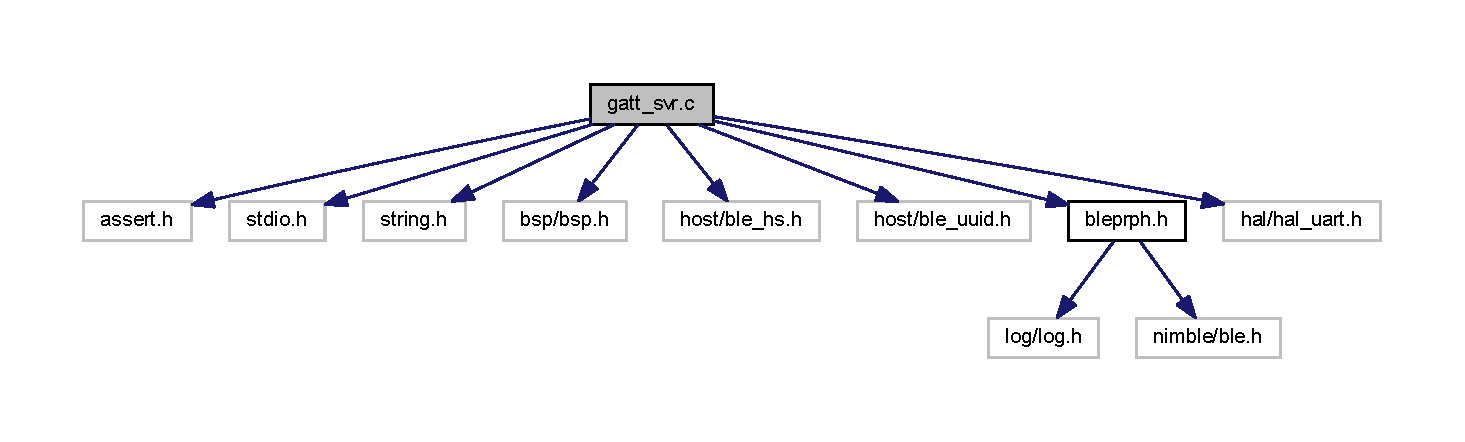
\includegraphics[width=350pt]{gatt__svr_8c__incl}
\end{center}
\end{figure}
\subsection*{Macros}
\begin{DoxyCompactItemize}
\item 
\#define \hyperlink{gatt__svr_8c_aeca034f67218340ecb2261a22c2f3dcd}{B\+U\+F\+S\+I\+ZE}~100
\end{DoxyCompactItemize}
\subsection*{Functions}
\begin{DoxyCompactItemize}
\item 
void \hyperlink{gatt__svr_8c_a1b1de510b8ab4e2449ccc2b3bd58461a}{gatt\+\_\+svr\+\_\+register\+\_\+cb} (struct ble\+\_\+gatt\+\_\+register\+\_\+ctxt $\ast$ctxt, void $\ast$arg)
\item 
int \hyperlink{gatt__svr_8c_a038a9dbf2f9610d386dbf69ea810aa9c}{gatt\+\_\+svr\+\_\+init} (void)
\end{DoxyCompactItemize}


\subsection{Macro Definition Documentation}
\mbox{\Hypertarget{gatt__svr_8c_aeca034f67218340ecb2261a22c2f3dcd}\label{gatt__svr_8c_aeca034f67218340ecb2261a22c2f3dcd}} 
\index{gatt\+\_\+svr.\+c@{gatt\+\_\+svr.\+c}!B\+U\+F\+S\+I\+ZE@{B\+U\+F\+S\+I\+ZE}}
\index{B\+U\+F\+S\+I\+ZE@{B\+U\+F\+S\+I\+ZE}!gatt\+\_\+svr.\+c@{gatt\+\_\+svr.\+c}}
\subsubsection{\texorpdfstring{B\+U\+F\+S\+I\+ZE}{BUFSIZE}}
{\footnotesize\ttfamily \#define B\+U\+F\+S\+I\+ZE~100}



\subsection{Function Documentation}
\mbox{\Hypertarget{gatt__svr_8c_a038a9dbf2f9610d386dbf69ea810aa9c}\label{gatt__svr_8c_a038a9dbf2f9610d386dbf69ea810aa9c}} 
\index{gatt\+\_\+svr.\+c@{gatt\+\_\+svr.\+c}!gatt\+\_\+svr\+\_\+init@{gatt\+\_\+svr\+\_\+init}}
\index{gatt\+\_\+svr\+\_\+init@{gatt\+\_\+svr\+\_\+init}!gatt\+\_\+svr.\+c@{gatt\+\_\+svr.\+c}}
\subsubsection{\texorpdfstring{gatt\+\_\+svr\+\_\+init()}{gatt\_svr\_init()}}
{\footnotesize\ttfamily int gatt\+\_\+svr\+\_\+init (\begin{DoxyParamCaption}\item[{void}]{ }\end{DoxyParamCaption})}

\mbox{\Hypertarget{gatt__svr_8c_a1b1de510b8ab4e2449ccc2b3bd58461a}\label{gatt__svr_8c_a1b1de510b8ab4e2449ccc2b3bd58461a}} 
\index{gatt\+\_\+svr.\+c@{gatt\+\_\+svr.\+c}!gatt\+\_\+svr\+\_\+register\+\_\+cb@{gatt\+\_\+svr\+\_\+register\+\_\+cb}}
\index{gatt\+\_\+svr\+\_\+register\+\_\+cb@{gatt\+\_\+svr\+\_\+register\+\_\+cb}!gatt\+\_\+svr.\+c@{gatt\+\_\+svr.\+c}}
\subsubsection{\texorpdfstring{gatt\+\_\+svr\+\_\+register\+\_\+cb()}{gatt\_svr\_register\_cb()}}
{\footnotesize\ttfamily void gatt\+\_\+svr\+\_\+register\+\_\+cb (\begin{DoxyParamCaption}\item[{struct ble\+\_\+gatt\+\_\+register\+\_\+ctxt $\ast$}]{ctxt,  }\item[{void $\ast$}]{arg }\end{DoxyParamCaption})}


\hypertarget{main_8c}{}\section{main.\+c File Reference}
\label{main_8c}\index{main.\+c@{main.\+c}}
{\ttfamily \#include $<$assert.\+h$>$}\newline
{\ttfamily \#include $<$string.\+h$>$}\newline
{\ttfamily \#include $<$stdio.\+h$>$}\newline
{\ttfamily \#include $<$errno.\+h$>$}\newline
{\ttfamily \#include \char`\"{}sysinit/sysinit.\+h\char`\"{}}\newline
{\ttfamily \#include \char`\"{}bsp/bsp.\+h\char`\"{}}\newline
{\ttfamily \#include \char`\"{}os/os.\+h\char`\"{}}\newline
{\ttfamily \#include \char`\"{}hal/hal\+\_\+gpio.\+h\char`\"{}}\newline
{\ttfamily \#include \char`\"{}console/console.\+h\char`\"{}}\newline
{\ttfamily \#include \char`\"{}hal/hal\+\_\+system.\+h\char`\"{}}\newline
{\ttfamily \#include \char`\"{}config/config.\+h\char`\"{}}\newline
{\ttfamily \#include \char`\"{}split/split.\+h\char`\"{}}\newline
{\ttfamily \#include \char`\"{}nimble/ble.\+h\char`\"{}}\newline
{\ttfamily \#include \char`\"{}host/ble\+\_\+hs.\+h\char`\"{}}\newline
{\ttfamily \#include \char`\"{}services/gap/ble\+\_\+svc\+\_\+gap.\+h\char`\"{}}\newline
{\ttfamily \#include \char`\"{}bleprph.\+h\char`\"{}}\newline
Include dependency graph for main.\+c\+:
\nopagebreak
\begin{figure}[H]
\begin{center}
\leavevmode
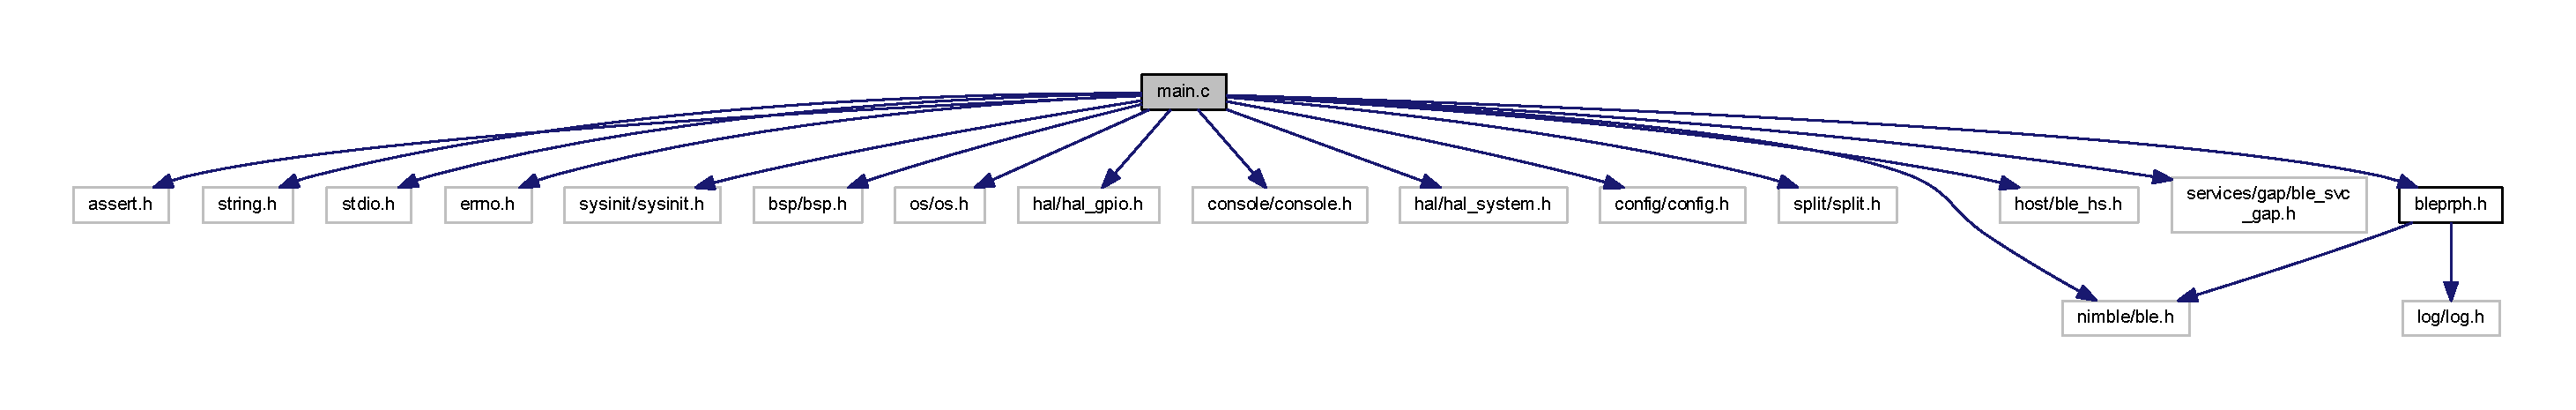
\includegraphics[width=350pt]{main_8c__incl}
\end{center}
\end{figure}
\subsection*{Functions}
\begin{DoxyCompactItemize}
\item 
int \hyperlink{main_8c_a840291bc02cba5474a4cb46a9b9566fe}{main} (void)
\end{DoxyCompactItemize}
\subsection*{Variables}
\begin{DoxyCompactItemize}
\item 
struct log \hyperlink{main_8c_a3cb7621a683b5c12e82853697f64aafb}{bleprph\+\_\+log}
\end{DoxyCompactItemize}


\subsection{Function Documentation}
\mbox{\Hypertarget{main_8c_a840291bc02cba5474a4cb46a9b9566fe}\label{main_8c_a840291bc02cba5474a4cb46a9b9566fe}} 
\index{main.\+c@{main.\+c}!main@{main}}
\index{main@{main}!main.\+c@{main.\+c}}
\subsubsection{\texorpdfstring{main()}{main()}}
{\footnotesize\ttfamily int main (\begin{DoxyParamCaption}\item[{void}]{ }\end{DoxyParamCaption})}

main

The main task for the project. This function initializes the packages, then starts serving events from default event queue.

\begin{DoxyReturn}{Returns}
int N\+O\+TE\+: this function should never return! 
\end{DoxyReturn}


\subsection{Variable Documentation}
\mbox{\Hypertarget{main_8c_a3cb7621a683b5c12e82853697f64aafb}\label{main_8c_a3cb7621a683b5c12e82853697f64aafb}} 
\index{main.\+c@{main.\+c}!bleprph\+\_\+log@{bleprph\+\_\+log}}
\index{bleprph\+\_\+log@{bleprph\+\_\+log}!main.\+c@{main.\+c}}
\subsubsection{\texorpdfstring{bleprph\+\_\+log}{bleprph\_log}}
{\footnotesize\ttfamily struct log bleprph\+\_\+log}

Log data. 
\hypertarget{misc_8c}{}\section{misc.\+c File Reference}
\label{misc_8c}\index{misc.\+c@{misc.\+c}}
{\ttfamily \#include \char`\"{}bleprph.\+h\char`\"{}}\newline
Include dependency graph for misc.\+c\+:
\nopagebreak
\begin{figure}[H]
\begin{center}
\leavevmode
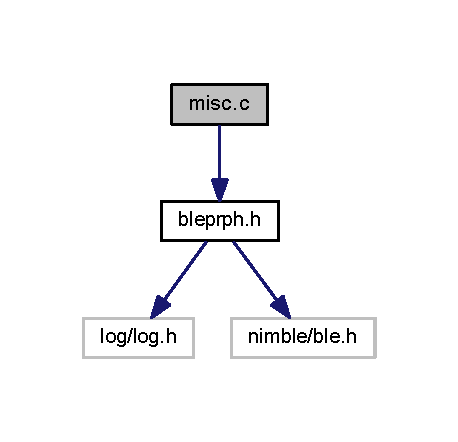
\includegraphics[width=220pt]{misc_8c__incl}
\end{center}
\end{figure}
\subsection*{Functions}
\begin{DoxyCompactItemize}
\item 
void \hyperlink{misc_8c_a3a0556a2cea77cb0defdfe38cbb4104d}{print\+\_\+bytes} (const uint8\+\_\+t $\ast$bytes, int len)
\item 
void \hyperlink{misc_8c_a03496a2baf54a46b40ea2000462f3291}{print\+\_\+addr} (const void $\ast$addr)
\end{DoxyCompactItemize}


\subsection{Function Documentation}
\mbox{\Hypertarget{misc_8c_a03496a2baf54a46b40ea2000462f3291}\label{misc_8c_a03496a2baf54a46b40ea2000462f3291}} 
\index{misc.\+c@{misc.\+c}!print\+\_\+addr@{print\+\_\+addr}}
\index{print\+\_\+addr@{print\+\_\+addr}!misc.\+c@{misc.\+c}}
\subsubsection{\texorpdfstring{print\+\_\+addr()}{print\_addr()}}
{\footnotesize\ttfamily void print\+\_\+addr (\begin{DoxyParamCaption}\item[{const void $\ast$}]{addr }\end{DoxyParamCaption})}

\mbox{\Hypertarget{misc_8c_a3a0556a2cea77cb0defdfe38cbb4104d}\label{misc_8c_a3a0556a2cea77cb0defdfe38cbb4104d}} 
\index{misc.\+c@{misc.\+c}!print\+\_\+bytes@{print\+\_\+bytes}}
\index{print\+\_\+bytes@{print\+\_\+bytes}!misc.\+c@{misc.\+c}}
\subsubsection{\texorpdfstring{print\+\_\+bytes()}{print\_bytes()}}
{\footnotesize\ttfamily void print\+\_\+bytes (\begin{DoxyParamCaption}\item[{const uint8\+\_\+t $\ast$}]{bytes,  }\item[{int}]{len }\end{DoxyParamCaption})}

Utility function to log an array of bytes. 
%--- End generated contents ---

% Index
\backmatter
\newpage
\phantomsection
\clearemptydoublepage
\addcontentsline{toc}{chapter}{Index}
\printindex

\end{document}
